%\part[Modelagem]{Modelagem}

\chapter{Modelagem do Sistema}

Como dito no capítulo 4, para se realizar a verificação do funcionamento do sistema, é necessário a simulação mista dos blocos analógicos com os blocos de controle digital, em específico um bloco de memória. Como a \textit{tag} envia, e recebe, dados em série, e um bloco de memória digital necessita de tais dados em paralelo, é necessário a modelagem de um conversor serial-paralelo, e um paralelo-serial para integrar o sistema.

O sistema digital idealizado e que foi modelado respeita então o seguinte diagrama de blocos:

\begin{figure}[ht!]
  \centering
  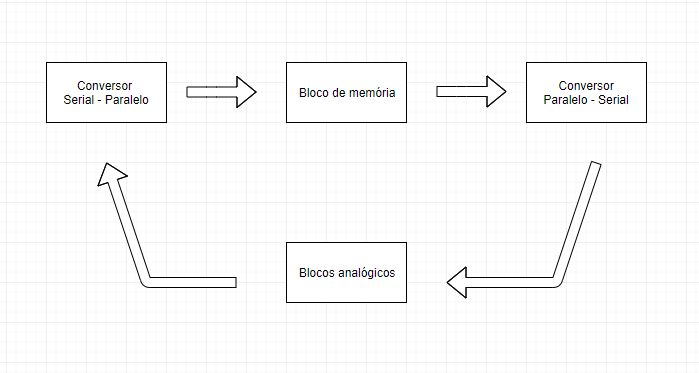
\includegraphics[width=\textwidth]{figuras/blocosmodelagem.JPG}
  \caption{Diagrama de blocos do sistema digital.}
  \label{bmodelagem}
\end{figure}

Neste capítulo, será abordado a modelagem destes blocos digitais e os procedimentos que foram realizados para a conexão destes blocos com os blocos analógicos, para que se fosse validada o funcionamento da
\textit{tag}. A escolha do tamanho da palavra de dados é arbitrária, porém, ela deve ser decidida antes da modelagem do sistema, pois todos os blocos devem ser devem usar um tamanho comum. Para a modelagem deste sistema, o tamanho da palavra de dados escolhido foi de quatro bits.

Todas as modelagens foram realizadas e simuladas utilizando a ferramenta Virtuoso, da Cadence.

\section{Modelagem do Conversor Serial Paralelo}

A figura \ref{verilogsp} mostra a modelagem do bloco conversor serial paralelo em verilog.

\begin{figure}[ht!]
  \centering
  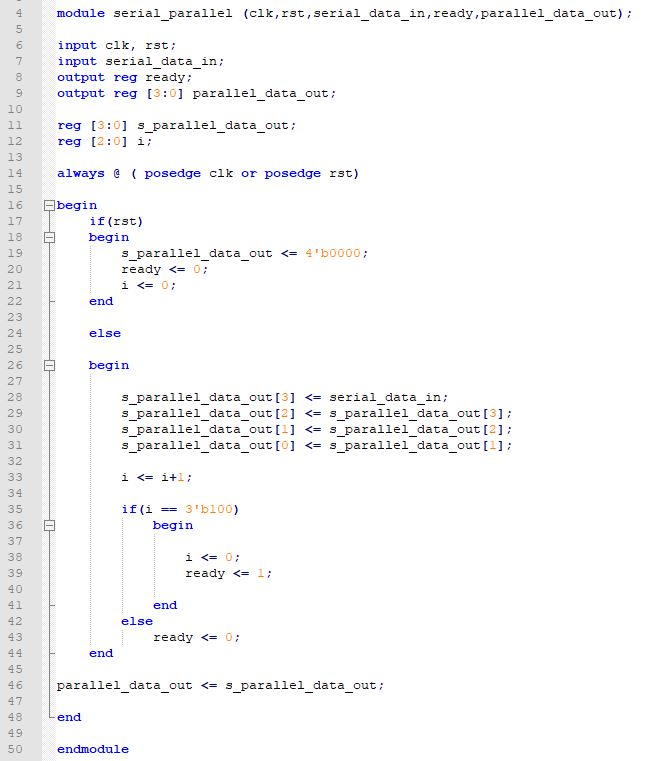
\includegraphics[width=0.8\textwidth]{figuras/verilogSP.JPG}
  \caption{Modelagem do bloco conversor serial paralelo.}
  \label{verilogsp}
\end{figure}

Este bloco possui três entradas (clk, rst e serial data in ) e duas saídas (ready e parallel data out). São utlizados também dois sinais de controle interno: 's parallel data out' e 'i'.

Através do comando "always @ (posedge clk or posedge rst)", realiza-se as operações designadas sempre que houver a borda de subida do sinal de clock ou de reset, em suas respectivas entradas. Caso o reset esteja em alto, o bloco voltará para o estado normal, zerando o sinal de entrada, os sinais de controle interno e a saída ready. Caso contrário, tem-se o funcionamento normal do bloco. 

Para se realizar a conversão serial paralelo, a cada subida de clock, ou seja, a cada bit do sinal serial enviado, há um shift na palavra de saída, que recebe este bit de entrada, e um incremento no sinal de controle 'i'. Este processo continua o número de vezes necessária para se adquirir todos os bits que formam a palavra desejada, no caso, de 4 bits. Neste momento, o sinal de controle 'i' é resetado, e o sinal 'ready' sinaliza para o bloco de memória que a palavra paralela está pronta para ser adquirida, esta palavra então será o endereço em que a memória irá buscar o dado solicitado.

\section{Modelagem do Bloco de Memória}

A figura \ref{verilogmem} mostra a modelagem do bloco de memória em verilog.

\begin{figure}[ht!]
  \centering
  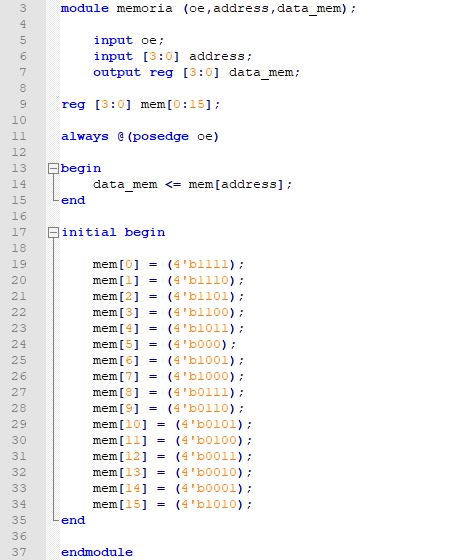
\includegraphics[width=0.8\textwidth]{figuras/verilogmem.JPG}
  \caption{Modelagem do bloco de memória.}
  \label{verilogmem}
\end{figure}

Este bloco é um bloco de memória simples, possui duas entradas (oe e address) e uma saída (data mem), possui também um sinal de controle interno (mem), onde são guardados dezesseis palavras de 4 bits.

Através do uso do comando 'always @ (posedge oe)' , pode-se realizar o resgate do valor armazenado no endereço recebido pela entrada 'address', atribuindo então ao sinal de saída (data men) o valor que foi resgatado no banco de dados da memória. Este comando será realizado sempre em que houver uma mudança de estado de 0 para 1 no sinal de controle 'oe' . 

O próximo passo no processo é converter o dado resgatado da memória em um sinal serial, já que é necessário que o modulador receba estes dados neste formado. Para tal é utilizado o bloco conversor paralelo serial.

\section{Modelagem do Conversor Paralelo Serial}

A figura \ref{verilogPS} mostra a modelagem do bloco conversor paralelo serial

\begin{figure}[ht!]
  \centering
  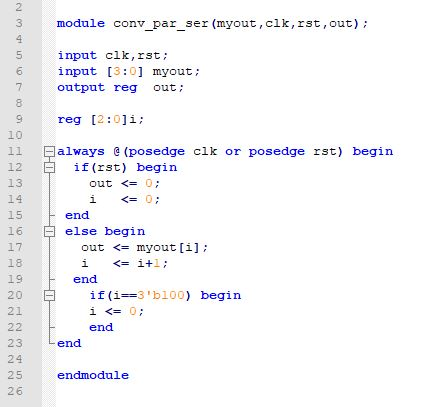
\includegraphics[width=0.8\textwidth]{figuras/verilogPS.JPG}
  \caption{Modelagem do bloco conversor paralelo serial.}
  \label{verilogPS}
\end{figure}

Este bloco possui três entradas (clk, rst e myout) e uma saída (out). além de um sinal interno de controle chamado 'i'.

Através do uso do comando 'Always @ (posedge clk or posedge rst)', realiza-se a conversão de paralelo para serial sempre que a borda de subida das entradas 'clk' e 'rst' são detectadas.

Caso a entrada de reset (rst) esteja ativa, a saída e o sinal de controle interno 'i' irão para 0. Se não for este o caso, a saída receberá o bit indexado na posição 'i' do vetor 'myout' e o sinal 'i' será incrementado. O processo será repetido até que o sinal 'i' alcance o valor do tamanho predeterminado da palavra (no caso, quatro), e será então resetado para converter a próxima palavra.

\section{Conexão Entre os Blocos Digitais e Analógicos}

Após a modelagem dos blocos digitais, foi realizada a conexão aos blocos analógicos para que se possa ser executada a validação do funcionamento da \textit{tag}. A ferramenta utilizada para este procedimento foi o 
Virtuoso da Cadence. 

Os blocos digitais foram incorporados ao projeto da \textit{tag} que possuiam os blocos analógicos e tiveram sua vista 'simbolo' geradas automaticamente após validado e compilado seu código verilog.

\begin{figure}[ht!]
  \centering
  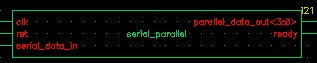
\includegraphics[width=0.8\textwidth]{figuras/blocosp.jpg}
  \caption{Vista símbolo gerada pelo Virtuoso.}
  \label{blocosp}
\end{figure}

\begin{figure}[ht!]
  \centering
  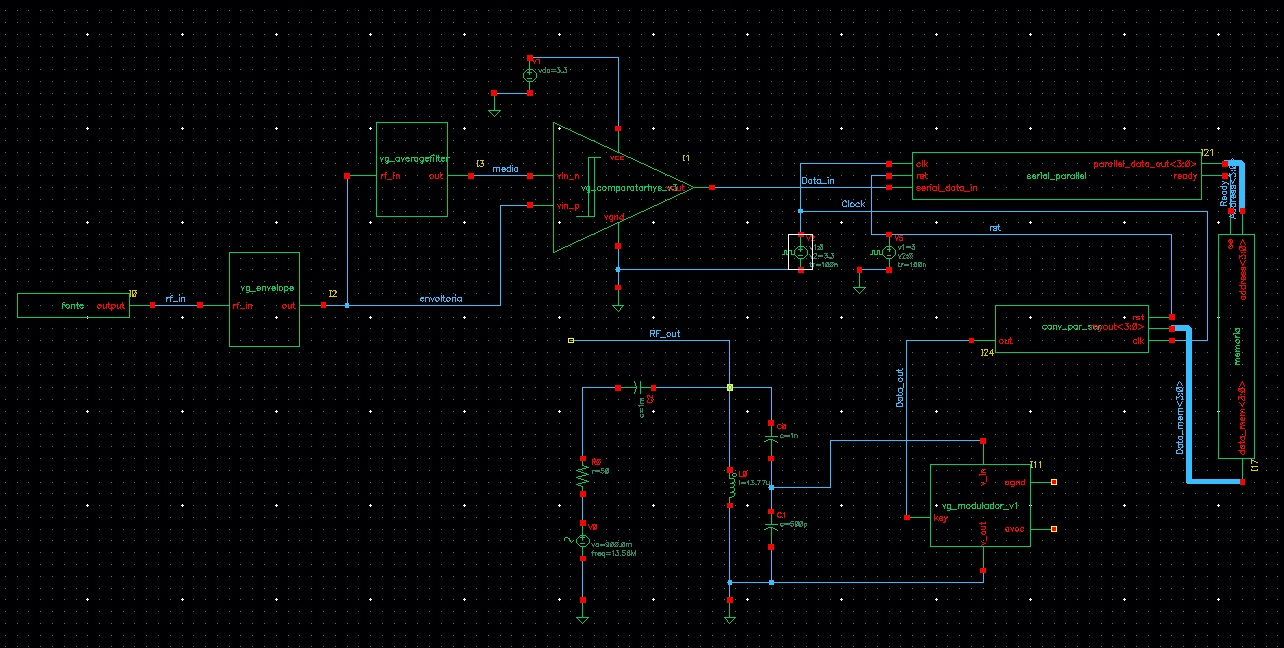
\includegraphics[width=\textwidth]{figuras/todosblocos.jpg}
  \caption{Esquemático completo da \textit{tag}.}
  \label{todosblocos}
\end{figure}

No proxímo passo, abre-se a vista de esquemático do projeto, utilizando a sub-ferramenta Schematic L, e se adiciona os blocos cujo quais serão interconectados para ser realizada a simulação completa da \textit{tag}.
São estes: Os blocos analógicos (Modulador, Demodulador e seus componentes), os blocos digitais (Conversor serial paralelo, memória e conversor paralelo serial), o bloco de fonte RF e outros componentes.

Para se conectar os blocos, é utilizado o componente 'wire (narrow)' para conexões simples, e 'wire (wide)' para conexões de vários bits. A conexão completa de todos os blocos da \textit{tag} pode ser vista na figura \ref{todosblocos}.

É importante frisar que os blocos analógicos foram estanciados em trabalhos anteriores, mais especificamente em \cite{Marlon}, bastando então realizar as conexões internas do bloco analógico, as conexões internas do bloco digital e a conexão entre os dois blocos. Com o esquemático completamente conectado, é feita então a simulação mista final.

